\documentclass{beamer}
\usepackage[latin1]{inputenc}
\usepackage[swedish,english]{babel}
\usepackage{amsmath,amssymb,mathtools,beamerthemesplit,mycommands}

% s/\\pgfqpoint{\([^}]*\)}{\([^}]*\)}/(\1,\2)/g
% s/\\pgfpathmoveto{\([^}]*\)}/\1/g
% s/\\pgfpathcurveto{\([^}]*\)}{\([^}]*\)}{\([^}]*\)}/ .. controls \1 and \2 .. \3/g
% s/\\pgfpathlineto{\([^}]*\)}/ -- \1/g
% s/\\pgfpathclose/ -- cycle/g

%%%%%%%%%%%%%%%%% Defining the theme %%%%%%%%%%%%%%%%%%%
\mode<presentation>
\definecolor{chalmersblue}{rgb}{0,0.2,0.53}
\setbeamercolor*{normal text}{fg=black,bg=white}
\setbeamercolor*{example text}{fg=chalmersblue}
\setbeamercolor*{structure}{fg=chalmersblue}
\setbeamercolor{palette primary}{use={structure,normal text},fg=white,bg=chalmersblue}
\setbeamercolor{palette secondary}{use={structure,normal text},fg=white,bg=black}
\setbeamercolor*{head}{parent=palette secondary}
\setbeamercolor*{foot}{parent=palette primary}
\defbeamertemplate*{footline}{chalmers theme}
{
  \leavevmode\hbox{%
  \begin{beamercolorbox}[wd=0.5\paperwidth,ht=2.25ex,dp=1ex,left]{foot}
   \usebeamerfont{foot}\hspace*{2ex}\insertsectionhead\ -\ \insertsubsectionhead\ -\ \insertsubsubsectionhead% This one you may want to comment
  \end{beamercolorbox}%
  \begin{beamercolorbox}[wd=0.25\paperwidth,ht=2.25ex,dp=1ex,left]{foot}
   \usebeamerfont{foot}\hspace*{2ex}\insertshortauthor%
  \end{beamercolorbox}%
  \begin{beamercolorbox}[wd=0.25\paperwidth,ht=2.25ex,dp=1ex,right]{foot}
   \usebeamerfont{foot}%
   \insertshortdate\hspace*{2ex}\insertframenumber/\inserttotalframenumber\hspace*{2ex}%
  \end{beamercolorbox}}\vskip0pt
}
\defbeamertemplate*{headline}{chalmers theme}
{
  \leavevmode\hbox{\begin{beamercolorbox}[wd=\paperwidth,ht=2.5ex,dp=1.5ex,left]{head}%
    \vspace{-.5ex}\hspace{2ex}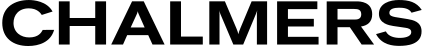
\includegraphics[height=2ex]{figures/Logo.pdf}%
  \end{beamercolorbox}}\vskip0pt
}
\setbeamersize{text margin left=1em,text margin right=1em}
\usenavigationsymbolstemplate{}
\floatsep=5mm
\abovecaptionskip=-1mm
\belowcaptionskip=-1mm

%%%%%%%%%%%%%%%%%%%%%%%%%%%% DOCUMENT START %%%%%%%%%%%%%%%%%%%%%%%%%%%%%%
\title{Stability of High Speed Train\\ under Aerodynamic Excitations}
\author{Erik Bjerklund \and Mikael �hman}
\begin{document}

\section{Title page} % Sections are shown at the bottom left. There is also links in many pdf-readers
\begin{frame}
 \titlepage
\end{frame}

\begin{frame}
 \frametitle{Acknowledgements}
 We would like to say our thanks to
\begin{itemize}
 \item Department of Applied Mechanics
 \item Supervisors Sini\v{s}a Krajnovi\'{c} and Viktor Berbyuk, and Albin Johnsson
 \item CFD support and Fire licenses from AVL\\ with a special thanks to Dr. Branislav Basara 
\end{itemize}
\end{frame}

\begin{frame}
 \frametitle{Purpose and goal}
 \begin{itemize}
  \item To investigate the stability and comfort of riding a high speed train.
  \item For the vibration dynamics to have reasonably good aerodynamic data.
  \item Usage of moving meshes for doing CFD.
  \item Two scenarios; meeting trains and train coming out of tunnel with side wind.
  \item Low order mathematical model. Modular framework with functional components.
  \item Look at the sensitivity to speed and look at the effects of active damping, especially in the coupling.
 \end{itemize}
\end{frame}

\section{Fluid mechanics}
\begin{frame}
 \frametitle{Two scenarios}
 \begin{itemize}
  \item Two trains meeting in the open at 140 m/s.
  \item Train coming out of tunnel under influence of a wind gust.
 \end{itemize}
  \begin{figure}
	\centering
% 	\includegraphics[height=0.33\textwidth]{figures/CFD/Phlash3.png}
% 	\includegraphics[height=0.33\textwidth]{figures/COVER_8.png}
	\caption{Aerodynamic effects influencing the train.}
  \end{figure}
\end{frame}

\subsection{CFD}
\begin{frame}
 \frametitle{CFD Calculations}
 \begin{itemize}
  \item Turbulence model, k-$\zeta$-f.
  \item Compressible flow.
  \item Unstructured mesh around train.
    \begin{figure}
	\centering
% 	\includegraphics[width=0.45\textwidth]{figures/CFD/Top_1.pdf}
% 	\includegraphics[width=0.5\textwidth]{figures/CFD/Train_2.pdf}
	\caption{Topology of mesh.}
  \end{figure}
 \end{itemize}
\end{frame}

\begin{frame}
 \frametitle{Moving mesh}
 \begin{itemize}
  \item Meshdeformation with sliding interface.
  \item Special boundary conditions.
  \item Dark blue and yellow regions are deformed on the left.
  \item Purple regions are deformed on the right.
  \begin{figure}
	\centering
% 	\includegraphics[width=0.45\textwidth]{figures/CFD/Move_mesh_6.jpg}
% 	\includegraphics[width=0.45\textwidth]{figures/CFD/F_24_printout/Mesh_slide_3.png}\\
% 	\includegraphics[width=0.45\textwidth]{figures/CFD/Move_mesh_5.jpg}
% 	\includegraphics[width=0.45\textwidth]{figures/CFD/F_24_printout/Mesh_slide_2.png}\\
% 	\includegraphics[width=0.45\textwidth]{figures/CFD/Move_mesh_4.jpg}
% 	\includegraphics[width=0.45\textwidth]{figures/CFD/F_24_printout/Mesh_slide.png}
	\caption{Moving mesh. Meeting trains on the left. Tunnel and train on the right.}
  \end{figure}
 \end{itemize}
\end{frame}

\subsection{Postproc Aero}
\begin{frame}
 \frametitle{Post-Processing}
 \begin{itemize}
  \item Forces and moments in each direction and around each axis.
  \item Forces and moments on split up between the cars.
  \item Pressure and shear forces.
  \end{itemize}
  \begin{figure}
	\centering
%         \includegraphics[width=0.45\textwidth]{figures/CFD/P_prints/pres_4.png}
% 	\includegraphics[width=0.45\textwidth]{figures/CFD/F_24_printout/pwin_4.png}\\
% 	\includegraphics[width=0.45\textwidth]{figures/CFD/P_prints/pres_6.png}
% 	\includegraphics[width=0.45\textwidth]{figures/CFD/F_24_printout/pwin_6.png}
	\caption{Relative pressure for, left, meeting trains, right, train and tunnel.}
  \end{figure}
\end{frame}

\begin{frame}
 \frametitle{Post-Processing cont.}
 \begin{itemize}
  \item Handed over to dynamic calculations
  \item Stars denote meeting and leaving trains on the left
  \item Stars denote start and end of exit of tunnel on the right.
  \end{itemize}
  \begin{figure}
	\centering
%         \includegraphics[width=0.49\textwidth]{figures/Fy_70_printout/Front_TT_2.pdf}
% 	\includegraphics[width=0.49\textwidth]{figures/Fy_70_printout/Front_QQ.pdf}
	\caption{The forces and moment on the front car}
  \end{figure}
\end{frame}

\section{Vibration dynamics}
\subsection{Workflow}
\begin{frame}
 \frametitle{Vibration dynamics workflow}
 \begin{figure}
  \centering
%   \includegraphics[width=\textwidth]{figures/model_block.pdf}
 \end{figure}
\end{frame}

\subsection{Bogie model}

\begin{frame}
 \frametitle{FLEXX Tronic Bogie}
 \begin{figure}
  \centering
%   \includegraphics[width=\textwidth]{figures/bogie/bogie_ref.jpg}
 \end{figure}
 \begin{itemize}
  \item Used in the REGINA 250 train.
  \item The most complex part of the train. Typically the part optimized for stability and comfort.
 \end{itemize}
\end{frame}

\begin{frame}
 \frametitle{Bogie model}
 \begin{figure}
  \centering
%   \includegraphics[scale=0.62]{MasterThesis-fig9.pdf}\hspace{2mm}
%   \includegraphics[scale=0.62]{MasterThesis-fig8.pdf}
 \end{figure}
 \begin{itemize}
  \item Constructed after the FLEXX Tronic bogie.
  \item No active damping included in the model.
  \item Assembled with train cars into a linear system.
 \end{itemize}
\end{frame}

\subsection{Vibrational Problem}
\begin{frame}
 \frametitle{Stability analysis}
 \begin{center}
  $L = \frac{\tan[\alpha]\mp\sgn[\phi_3] \mu}{1\pm\sgn[\phi_3] \mu \tan[\alpha]}$\hspace{10mm}
  $F_{s,i} = \left(\frac{F_{flange,i}}{N_{h,i} L_i}\right)^2$\hspace{10mm}
  $J_{s,1} = \sqrt{\frac{1}{t_1-t_0}\int_{t_0}^{t_1} \sum F_{s,i} dt}$\\
  $J_{s,2} = \sqrt{\frac{1}{t_1-t_0}\int_{t_0}^{t_1} \sum y_i^2 dt}$
 \end{center}
 \begin{itemize}
  \item Stability is analyzed through risk of wheel climb.
  \item Secondary measurement $J_{s,2}$ for cases when the flange doesn't touch the rail, i.e. when $J_{s,1}\equiv0$.
  \item $F_i$ and $y_i$ is calculated for each wheel.
  \item $J_{s,1}$ is dimensionless, $J_{s,2}$ is a RMS of the lateral displacement.
 \end{itemize}
\end{frame}

\begin{frame}
 \frametitle{Comfort analysis}
 \begin{center}
  $\uv{d} = \uv{x} + \uv{\varphi} \times \overrightarrow{\uv{v}} $
  \hspace{10mm}
  $F_i = |\uv{\ddot{d}}_i|^2$
  \hspace{10mm}
  $J_c = \sqrt{\frac{1}{t_1-t_0}\int_{t_0}^{t_1} \sum F_i dt}$
  \end{center}
 \begin{itemize}
  \item RMS of acceleration.
  \item $F_i$ is calculated for each corner of each train car.
  \item Lower $J_c$ is better.
  \item Worst for middle car.
 \end{itemize}
\end{frame}

\subsection{Difference}
\begin{frame}
 \frametitle{Difference between the scenarios.}
 \begin{itemize}
  \item Meeting trains: Vibrations in the car, insignificant impact on stability.
  \item Tunnel and side wind: Massive impact on stability.
 \end{itemize}
 \begin{table}[htpb!]
 \centering
 \caption{Absolute values of the stability and comfort measurements for both scenarios at 70 m/s.}
 \vskip 5mm
 \begin{tabular}{|r|r|r|r|}
  \hline                      & $J_c$ [m/s$^2$] & $J_{s,1}$ [-] &      $J_{s,2}$ [m]\\
  \hline Meeting trains       &          $0.66$ &        $0.00$ &   $4\times10^{-4}$\\
  \hline Tunnel and side wind &         $10.71$ &        $0.55$ & $245\times10^{-4}$\\
  \hline
 \end{tabular}
\end{table}
\end{frame}

\subsection{Speed sensitivity}
\begin{frame}
 \frametitle{Speed sensitivity}
 \begin{figure}
  \centering
%   \includegraphics[width=0.49\textwidth]{figures/speeds/TT_0312.pdf}
%   \includegraphics[width=0.49\textwidth]{figures/speeds/QQ_0409.pdf}
  \caption{Less is better. Linear behaviour even though loads are strongly nonlinear.}
 \end{figure}
 Data is extrapolated for scenario with tunnel, assuming constant lift coefficient.
\end{frame}

\begin{frame}
 \frametitle{Optimization, Meeting Trains}
 Less is better. $J_c$ and $J_s$ are strongly correlated.
 \begin{figure}
  \centering
%   \includegraphics[width=0.49\textwidth]{figures/optimization/k2_c2_Jc_TT.pdf}
%   \includegraphics[width=0.49\textwidth]{figures/optimization/k2_c2_Js2_TT.pdf}
  \caption{Optimization of lateral spring and damper.}
 \end{figure}
\end{frame}

\begin{frame}
 \frametitle{Optimization, Tunnel and Side Wind}
 Again $J_c$ and $J_s$ are strongly correlated, but a very different optimization criterion from meeting trains.
 \begin{figure}
  \centering
%   \includegraphics[width=0.49\textwidth]{figures/optimization/k2_c2_Jc_QQ.pdf}
%   \includegraphics[width=0.49\textwidth]{figures/optimization/k2_c2_Js1_QQ.pdf}
  \caption{Optimization of lateral spring and damper.}
 \end{figure}
\end{frame}

\begin{frame}
 \frametitle{Optimization, Both}
 Using $k_y$ = 50 kN/m, $c_y$ = 700 kNs/m (meeting trains), $c_y$ = 100 kNs/m (tunnel and side wind).
 \begin{figure}
  \centering
%   \includegraphics[width=0.49\textwidth]{figures/optimization/c4_TT.pdf}
%   \includegraphics[width=0.49\textwidth]{figures/optimization/c4_QQ.pdf}
 \end{figure}
 Minimum at $c_{roll}\approx$ 20 kNsm.
\end{frame}

\subsection{Semi-Active Damping}
\begin{frame}
 \frametitle{Sky-Hook and Ground-Hook dampers}
 \begin{figure}
 \centering
%  \includegraphics[width=0.33\textwidth]{figures/skyhook/skyhook_TT.pdf}
%  \includegraphics[width=0.33\textwidth]{figures/skyhook/skyhook_QQ.pdf}\\
%  \includegraphics[width=0.33\textwidth]{figures/skyhook/groundhook_TT.pdf}
%  \includegraphics[width=0.33\textwidth]{figures/skyhook/groundhook_QQ.pdf}
 \end{figure}
 \begin{itemize}
  \item $c_{min}=f\times c_{max}$
  \item Very minor improvements, mostly far worse.
 \end{itemize}
\end{frame}

\begin{frame}
\frametitle{Collected results}
\begin{table}
 \caption{Comparison of the optimized values.}
 \vskip 1mm
 \label{tab:passive_opt_results}
 \begin{tabular}{|l|r|r|r|}
  \hline                    & Initial         & Meeting trains & Tunnel and side win\\
  \hline $k_y$ [kN/m]       & 2$\times10^{4}$ &             50 &                  50\\
  \hline $c_y$ [kNs/m]      &             100 &            700 &                 100\\
  \hline $c_{roll}$  [kNsm] &               5 &             20 &                  20\\
  \hline Relative change of $J_c$      &      &        -7.82\% &             -7.18\%\\
  \hline Relative change of $J_{s,1}$  &      &                &             -4.58\%\\
  \hline Relative change of $J_{s,2}$  &      &        -0.55\% &             -8.88\%\\
  \hline Effect in speed               &      &  -3 to -4[m/s] &       -3 to -5[m/s]\\
  \hline
 \end{tabular}
\end{table}
\end{frame}
\section{End}
\begin{frame}
 \frametitle{Thanks!}
 \begin{center}
 \Large{Thank you for listening.}
 \end{center}
\end{frame}

\end{document}
